\chapter{Requirement specification}
\label{kravsspec}

Systemkrav

I dette kapitel opstilles en projektplan med en generel produktbeskrivelse og specifikke systemkrav. Projektplanen, produktbeskrivelsen og systemkravene formuleres for at produktet i sidste ende kommer til at fungere efter hensigten. Produktet beskrives først generelt ved hjælp af Use Cases. På baggrund af den generelle produktbeskrivelse formuleres en række specifikke systemkrav. De endelige krav vil til sidst opsummeres i prioriteret rækkefølge.

\section{Projektplan}
Projektet startes XX og forventes afsluttet XX. Ved afslutningen forventes en fungerende elektronisk prototype der kan symbolisere og viderformidle den tekniske løsning. Ved projektets afslutning forventes den elektroniske prototype ikke at fremstå som et færdigt produkt, men som en støtte til viderformidling af konceptet. Prototypen forventes at gennemgå en iterativ udvikling igennem hele projektperioden. 

\section{Generel produktbeskrivelse}
Målet for projektet er at udarbejder et elektronisk instrument, som kan simulere lyde fra et trommesæt. De forskellige trommelyde afspilles ved hjælp af fingerspidserne, hvor hver fingerspids har sin egen unikke lyd. En lyd afspilles når en finger laver en trommebevægelse. En trommebevægelse er en gestikulering hvor fingerspidsen rammer en overflade og derved møder modstand. Modstanden detekteres af en elektronisk sensor. En trommebevægelse kan derved laves på mange forskellige overflader, eksempelvist et bord, en væg eller et lårben. Brugeren af produktet vælger med fingerspidsernes sensorer hvilken lyd der skal afspilles og hvornår den skal afspilles.

Trommelydende kan i princippet varieres og skiftet ud efter brugerens ønske. Som udgangspunkt kan en unik lyd for hver fingerspids frembringes. Brugeren kan ved hjælp af et display udskifte eller omarrangere de unikke lyde efter behov. På den måde kan produktet tilpasses specifikke brugere samt brugssituationer. Brugeren kan ændre lydstyrken ved hjælp af displayet. Det er også ved hjælp af displayet at produktets tænd/sluk funktion tilgås. 

Produktet udformes som en handske der kan tages af og på. Sensorernes position fastholdes på fingerspidserne ved hjælp af handsken. Ideelt er det mulighed at integrere display og styresystem til produktet omkring håndledet ved handskens munding. Styresystem og display forventes at simuleres af en bærbar PC, hvorfor det af praktiske og ergonomiske årsager ikke forventes at integreres omkring håndledet. I stedet forventes information fra sensorerne at kommunikeres via fleksible ledning til et styresystemet. 

\section{Use Cases}
Følgende afsnit fokusere på de funktionelle krav som produktet skal opfylde. Produktets funktioner beskrives ved hjælp af Use Cases, hvor grænseflader mellem aktører og funktioner vil fremgå. Den generelle produktbeskrivelse lægger op til uddybelse af produktets funktionelle krav, samt en opdeling af de aktører, som indgår i processen.

Brugeren af produktet skal have mulighed for at afspille lyde, udskifte lyde, ændre lydstyrke samt tænde og slukke for systemet. Afspil lyd, Udskift lyd, Ændr lydstyrke og Tænd/sluk er derfor essentielle funktioner at implementere, for at produktet fungere optimalt. For at brugeren i sidste ende kan tilgå funktionerne er det nødvendigt at kende de interne og eksterne aktører som er involveret i  processerne. Som nævnt i ***section - Generel produktbeskrivelse*** er målet for projektet at fremstille en elektronisk prototype, som ved hjælp af et styresystem kan afspille forskellige trommelyde på baggrund af brugerens interaktion med sensorer og et display. De interne aktører; Sensorer, Display og Styresystem, symboliserer hvor der foregår en interaktion mellem produktets forskellige funktioner og aktører. Brugeren selv defineres som en ekstern aktør, ligsom højtaler, der i sidste ende afspiller lyden, også fremgår som eksterne aktører. Det sker for at simplificere Use Case diagrammet til kun at omfatte systemet selv. Use Case diagrammet på figur ***FIGUR AF USE CASE DIAGRAM*** fokusere derfor på de interne aktører, som gør funktionerne tilgængelige via grænsefladerne mellem funktion og aktør. 

\begin{figure}
\centering
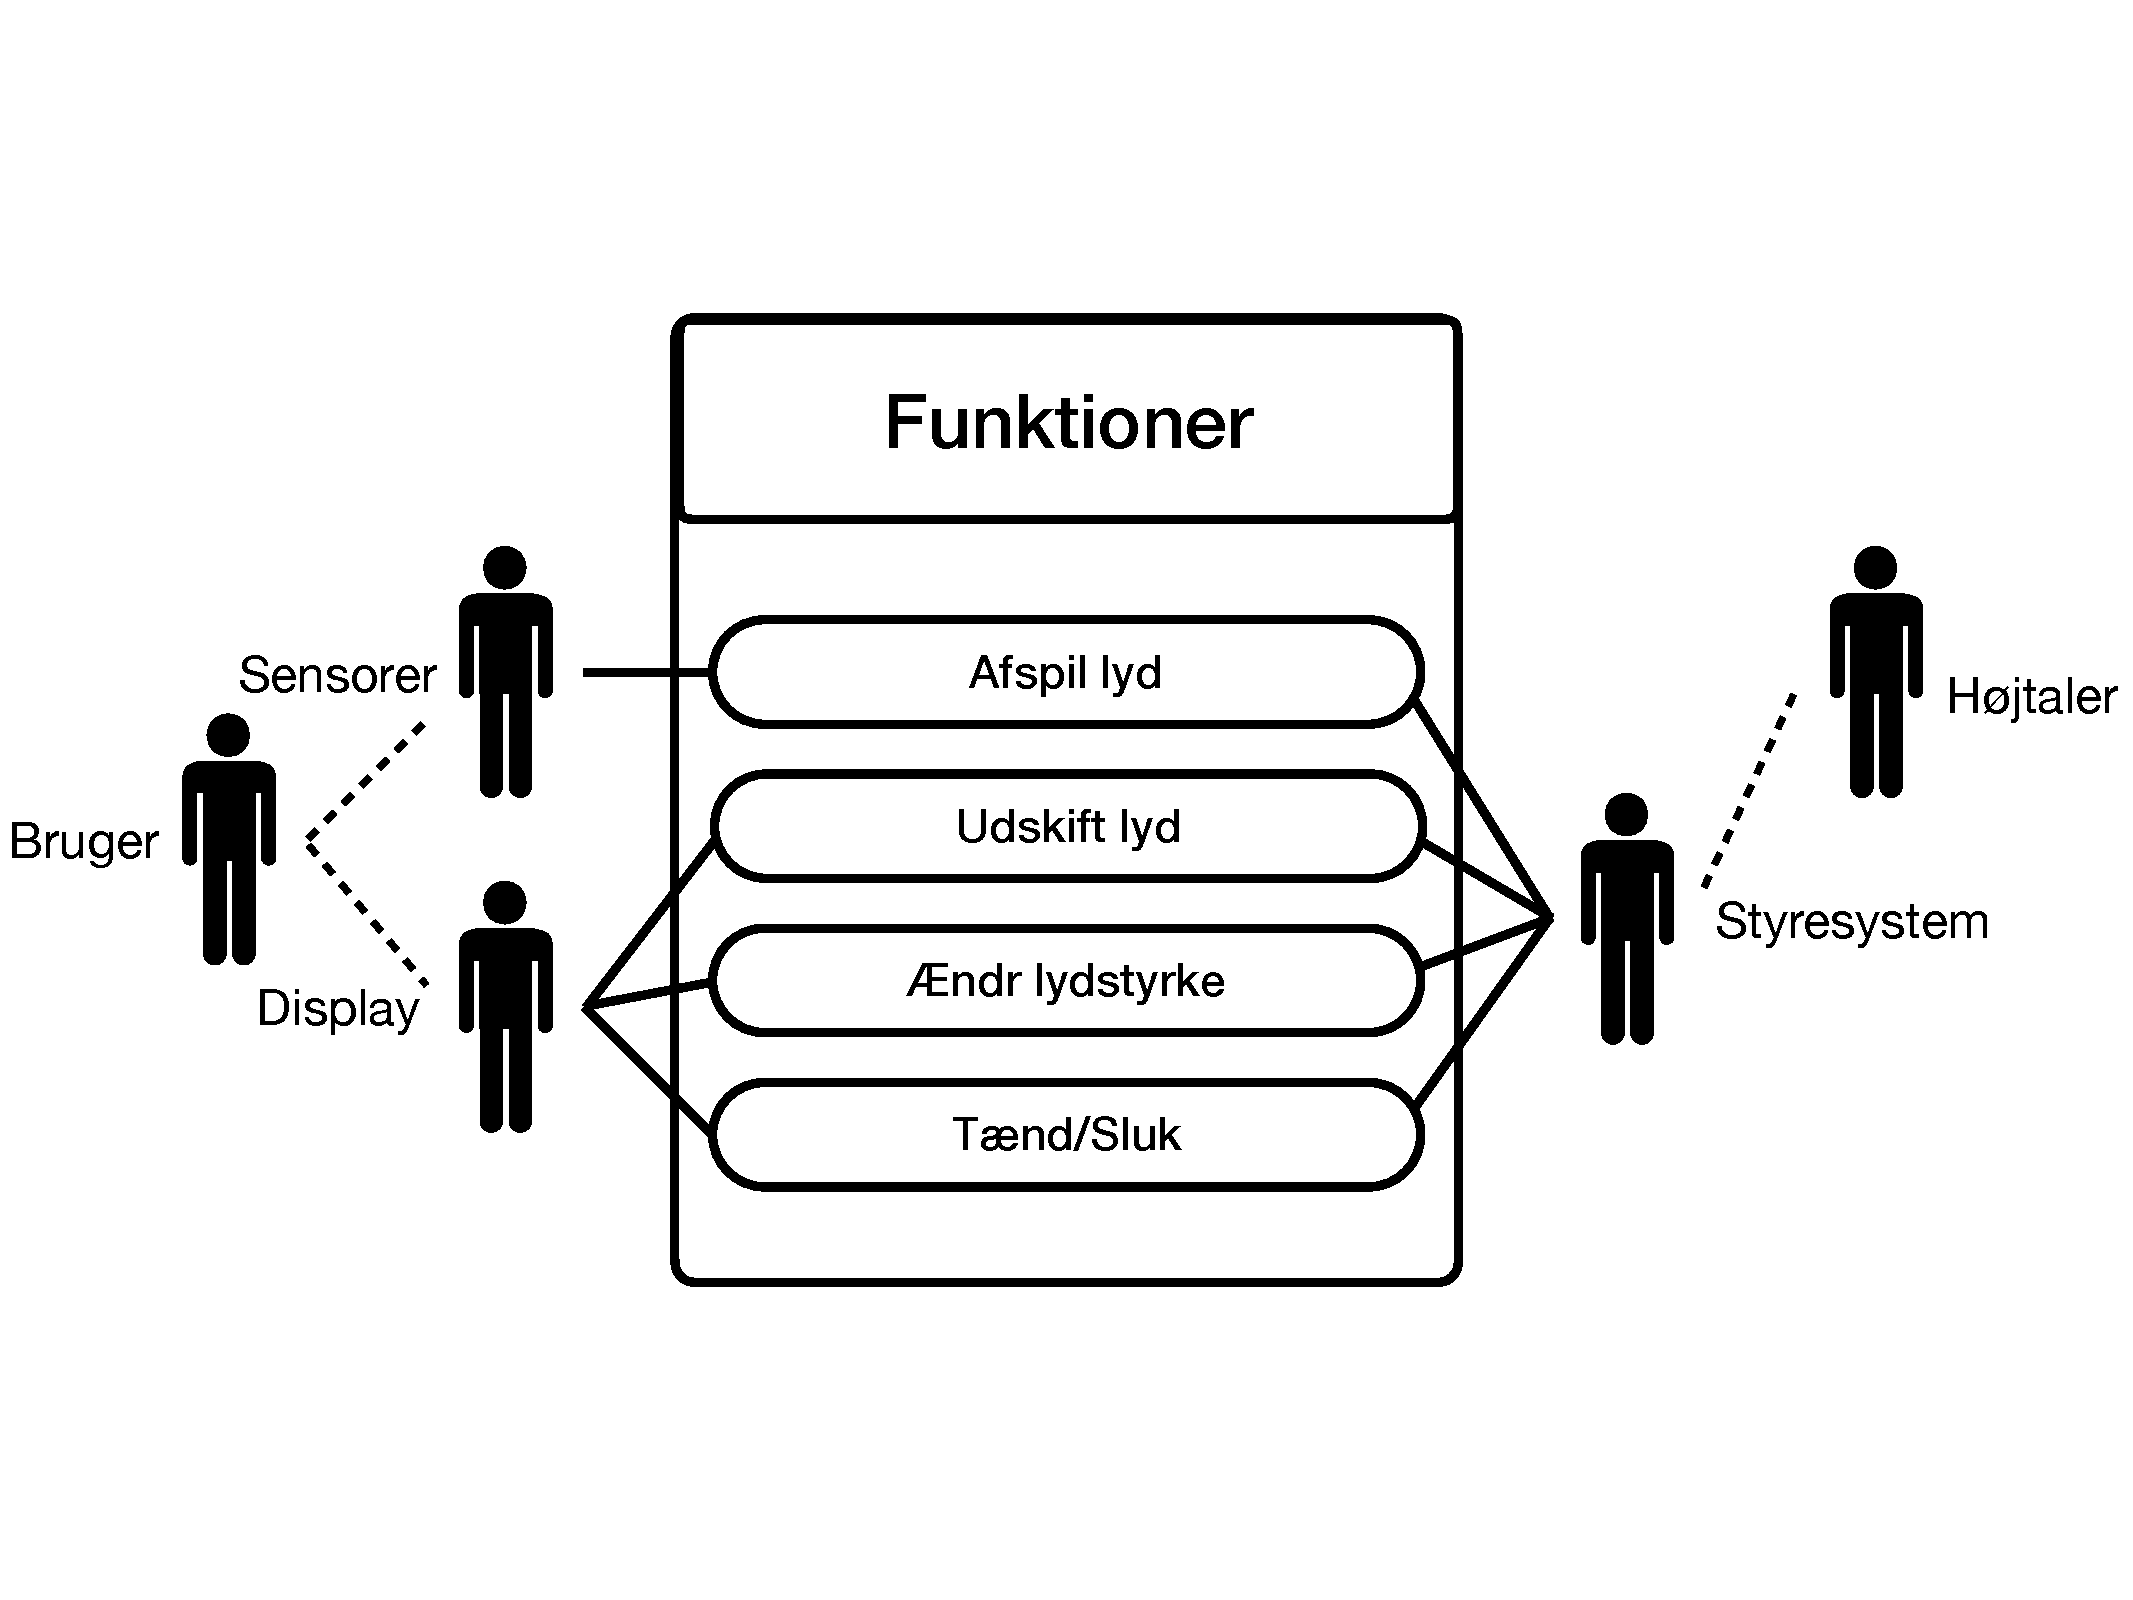
\includegraphics[scale=0.4]{Figure/protoUseCase}
\caption{
Use Case diagram for det samlede system. De fire Use Cases er forbundet til deres respektive aktører. Mellem Use Case og aktør findes grænsefladen, som er udtryk for hvilke aktører der kommunikere med hinanden.}
\label{fig:protoUseCase}
\end{figure}

\subsection{Afspil lyd}
Brugeren interagere med sensorerne for at afspille en unik trommelyd. Sensorerne signalere, via grænsefladen til styresystemet, at en finger laver en trommebevægelse. Styresystemet reagere på signalet og interagere med den eksterne aktør, højtaler, der derefter afspiller lyden.    

\subsection{Udskift lyd}
Brugeren interagere med displayet for at udskifte eller omarrangere en lyd. Displayet signalere, via grænsefladen til styresystemet, at en lyd skal ændres. Styresystemet reagere på signalet og ændre derefter den respektive lyd.   

\subsection{Ændr lydstyrke}
Brugeren interagere med displayet for at ændre lydstyrken. Displayet signalere, via grænsefladen til styresystemet, at lydstyrken skal ændres. Styresystemet reagere på signalet og ændre derefter lydstyrken. 

\subsection{Tænd/sluk}
Brugeren interagere med displayet for at tænde eller slukke systemet. Displayet signalere, via grænsefladen til styresystemet, at systemet enten skal tændes eller slukkes. Styresystemet reagere på signalet, hvorefter systemet enten tænder eller slukker




-----------------------------

Hovedfunktioner: 
Begrænsninger:
Brugerprofiler:

Specifikke krav: 
Sensorene skal kunne signalere om en respektiv finger trommer eller ej. 
Styringsenheden skal kunne aflæse signalet fra sensorerne, behandler signalet og afspille en lydfil til en højtaler.

… detailkrav/
ydelseskrav/
kvalitetskrav/
designkrav      

 
